\begin{frame}[allowframebreaks]{Text-to-SVG}
    \begin{itemize}
        \item Text-to-SVG generation is a novel application of diffusion models, enabling the creation of vector graphics from textual descriptions.
        \item The process involves training a diffusion model to learn the distribution of SVG images conditioned on text prompts.
        \item The model generates SVG paths, which are inherently vector-based and scalable without loss of quality.
    \end{itemize}
    \framebreak
    
    \begin{itemize}
        \item Using SDS loss is not limited to text-to-3D.
        \item SDS provides a general way to backpropagate and learn through any differentiable “rendering” pipeline.
    \end{itemize}
    \begin{figure}
        \centering
        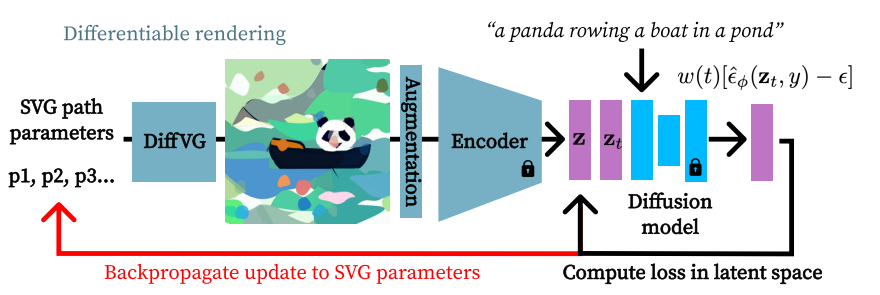
\includegraphics[width=1.05\linewidth,height=\textheight,keepaspectratio]{images/adv-img-gen/slide_160_1_img.png}
        \caption*{Jain, Ajay, Amber Xie, and Pieter Abbeel. "Vectorfusion: Text-to-svg by abstracting pixel-based diffusion models." Proceedings of the IEEE/CVF Conference on Computer Vision and Pattern Recognition. 2023.}
    \end{figure}

    \framebreak
    \begin{figure}
        \centering
        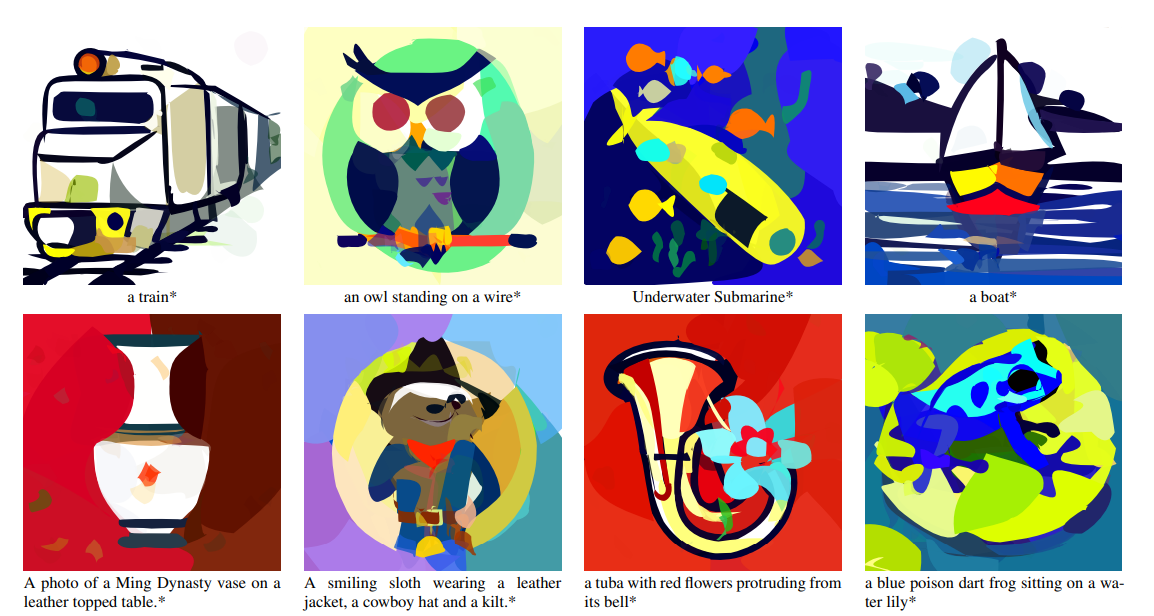
\includegraphics[width=1.05\linewidth,height=\textheight,keepaspectratio]{images/adv-img-gen/slide_161_1_img.png}
    \end{figure}
\end{frame}